\documentclass[11pt]{report}

\usepackage{geometry,amsmath,amssymb,amsthm}

\usepackage{enumerate}

\usepackage{tikz,pgfplots}

\geometry{margin=1.in}

\theoremstyle{plain}
\newtheorem{thm}{Theorem}
\newtheorem{lem}[thm]{Lemma}
\newtheorem{prop}[thm]{Proposition}
\newtheorem{cor}[thm]{Corollary}

\newcommand{\ds}{\displaystyle}


\begin{document}
\hfill Math 251 Calculus I
\begin{center}
\Large{\textbf{Written Homework Problems \S 5.1}} \\
5 problems for 10 points\\
\end{center}

\begin{description}
\item{\S 5.1} \#(12,14,15)**, 35, 39\\

** For all of these problems, use technology to draw the graph of the function over the given interval. Add to your graph the rectangles corresponding the left- or right-handed sums. For each example, decide if you think your estimate is an over-estimate, an underestimate, or hard to determine.
\end{description}

{\bf Additional Problems.} Remember that we are computing the \emph{signed area} between a curve and the $x$-axis. If the area is below the $x$-axis, then the sign of the area is negative, and if the area is above the $x$-axis then the sign of the area is positive.

\begin{enumerate}[{\bf {Problem} A.}]
\item A portion of the piecewise-linear function \[f(x) = \begin{cases} 
-x&\quad x\leq 3\\
\frac{3}{2}(x-5) &\quad x > 3
\end{cases} \]
is graphed below.

\begin{center}
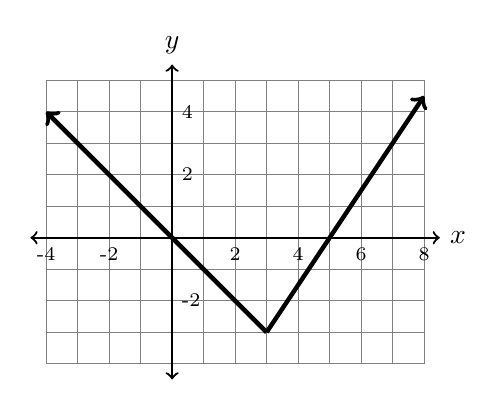
\begin{tikzpicture}[scale = .4]
%cubic
%\begin{axis}[xscale = 1, yscale = 1, thick, my style, xtick={-2,2,4,...,10}, ytick={-1,1,2,3,4},xmin=-5, xmax=10, ymin=-5, ymax=6, minor y tick num=1, minor x tick num=1, 
%mark size=3.0pt, grid = major, ]
%%\addplot[ultra thick, -,domain=-4:-2, samples=100, <-]coordinates {(-4,-2)(-2,2)};
%\addplot[ultra thick, domain=-5:5, samples=100, ,]{sqrt(25-x^2)};
%\addplot[ultra thick, ->,domain=5:9, samples=100]{-1/2*(x-5)};
%\end{axis}

\draw[help lines] (-4, -4) grid (8, 5);
\draw[thick,<->] (-4.5,0) -- (8.5,0) node[right] {$x$};
\draw[thick,<->] (0,-4.5) -- (0,5.5) node[above] {$y$};
\draw[ultra thick, ->] (3,-3) -- (8,3/2*8-3/2*5);
\draw[ultra thick, <-] (-4,4) -- (3,-3);
%\draw[ultra thick] (5,0) arc (0:180:5);
\foreach \i in { -4,-2,2,4,6,8} {\path  (\i,0)node[below, font = \scriptsize] {\i};}
\foreach \i in {-2,2,4} {\path  (0, \i)node[right, font = \scriptsize] {\i};}

\end{tikzpicture}
\end{center}
%\begin{enumerate}
Approximate $\ds \int_{-2}^{7} f(x) \ dx$ using three left-hand rectangles. {\bf Draw} the rectangles on the graph.
Then {\bf use geometry} to compute $\ds \int_{-2}^{7} f(x) \ dx$ exactly. %\vfill
%	\end{subproblems}

\item A portion of the function \[f(x) = \begin{cases} \sqrt{25-x^{2}} \quad -5 \leq x \leq 5 \\ -\frac{1}{2}(x-5) \quad x \geq 5
\end{cases} \]
is graphed below.

\begin{center}
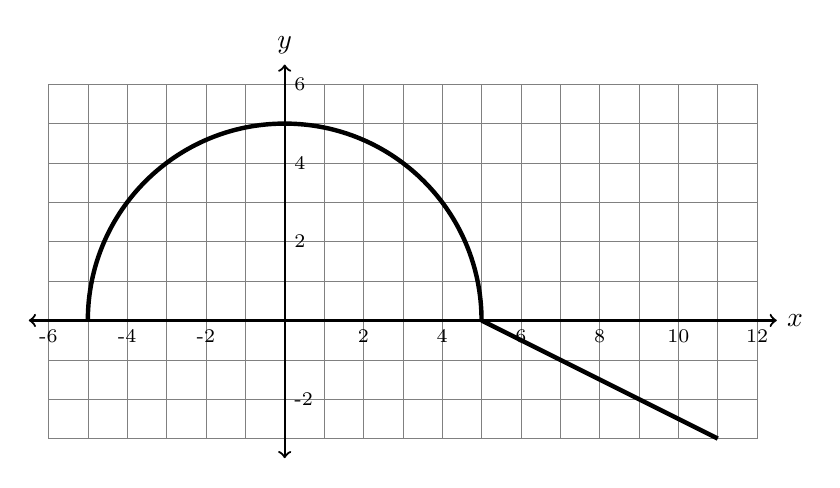
\begin{tikzpicture}[scale = .5]
%cubic
%\begin{axis}[xscale = 1, yscale = 1, thick, my style, xtick={-2,2,4,...,10}, ytick={-1,1,2,3,4},xmin=-5, xmax=10, ymin=-5, ymax=6, minor y tick num=1, minor x tick num=1, 
%mark size=3.0pt, grid = major, ]
%%\addplot[ultra thick, -,domain=-4:-2, samples=100, <-]coordinates {(-4,-2)(-2,2)};
%\addplot[ultra thick, domain=-5:5, samples=100, ,]{sqrt(25-x^2)};
%\addplot[ultra thick, ->,domain=5:9, samples=100]{-1/2*(x-5)};
%\end{axis}

\draw[help lines] (-6, -3) grid (12, 6);
\draw[thick,<->] (-6.5,0) -- (12.5,0) node[right] {$x$};
\draw[thick,<->] (0,-3.5) -- (0,6.5) node[above] {$y$};
\draw[ultra thick] (5,0) -- (11,-3);
\draw[ultra thick] (5,0) arc (0:180:5);
\foreach \i in {-6, -4,-2,2,4,6,8,10, 12} {\path  (\i,0)node[below, font = \scriptsize] {\i};}
\foreach \i in {-2,2,4,6} {\path  (0, \i)node[right, font = \scriptsize] {\i};}

\end{tikzpicture}
\end{center}


Approximate $\ds \int_{0}^{9} f(x) \ dx$ using three right-hand rectangles. Carefully draw the three right-hand rectangles on the graph. Lightly shade them in. Then use geometry to compute $\ds \int_{0}^{9} f(x) \ dx$ exactly. 

\item The function $f(x)=2-2 \ln(x)$ is graphed below. We want to estimate the area between the curve $f(x)$ and the $x$-axis on the interval $[1,9]$ using $L_4.$ (That is, we want to use 4 approximating rectangles and left-hand end points.)  Sketch the four approximating rectangles on the graph. Then do a calculation to estimate the area under the curve using $L_4$ (that is, use 4 approximating rectangles and left-hand end points) and simplify your answer.  \emph{Note: You are obviously not expected to compute things like $\ln(4)$ without a calculator. It is acceptable to have numbers like this in your final answer.} \\

\begin{tikzpicture}[scale=.8]
\draw[thick, ->] (0,-3) -- (0,4.8);
\draw[thick, ->] (-1,0) -- (10.2,0);
\foreach \j in { 1,2,3,4,5,6,7,8,9,10}{
	\draw (\j,-0.15) -- (\j, 0.15);
	\node at (\j,-.5){$\j$};
	}
\foreach \j in {-3,-2,-1,1,2,3,4}{
	\draw (-0.15,\j) -- (0.15,\j);
	\node at (-0.5,\j){$\j$};
	}
\draw[<->,line width=1.2pt,smooth,samples=100,domain=0.5:10] plot(\x,{2-2*ln((\x))});
\end{tikzpicture}






\end{enumerate}

\end{document}